%\documentclass[
  bibliography=totoc,     % Literatur im Inhaltsverzeichnis
  captions=tableheading,  % Tabellenüberschriften
  titlepage=firstiscover, % Titelseite ist Deckblatt
]{scrartcl}

% Paket float verbessern
\usepackage{scrhack}

% Warnung, falls nochmal kompiliert werden muss
\usepackage[aux]{rerunfilecheck}

% unverzichtbare Mathe-Befehle
\usepackage{amsmath}
% viele Mathe-Symbole
\usepackage{amssymb}
% Erweiterungen für amsmath
\usepackage{mathtools}

% Fonteinstellungen
\usepackage{fontspec}
% Latin Modern Fonts werden automatisch geladen
% Alternativ zum Beispiel:
%\setromanfont{Libertinus Serif}
%\setsansfont{Libertinus Sans}
%\setmonofont{Libertinus Mono}

% Wenn man andere Schriftarten gesetzt hat,
% sollte man das Seiten-Layout neu berechnen lassen
\recalctypearea{}

% deutsche Spracheinstellungen
\usepackage[ngerman]{babel}


\usepackage[
  math-style=ISO,    % ┐
  bold-style=ISO,    % │
  sans-style=italic, % │ ISO-Standard folgen
  nabla=upright,     % │
  partial=upright,   % │
  mathrm=sym,        % ┘
  warnings-off={           % ┐
    mathtools-colon,       % │ unnötige Warnungen ausschalten
    mathtools-overbracket, % │
  },                       % ┘
]{unicode-math}

% traditionelle Fonts für Mathematik
\setmathfont{Latin Modern Math}
% Alternativ zum Beispiel:
%\setmathfont{Libertinus Math}

\setmathfont{XITS Math}[range={scr, bfscr}]
\setmathfont{XITS Math}[range={cal, bfcal}, StylisticSet=1]

% Zahlen und Einheiten
\usepackage[
  locale=DE,                   % deutsche Einstellungen
  separate-uncertainty=true,   % immer Unsicherheit mit \pm
  per-mode=symbol-or-fraction, % / in inline math, fraction in display math
]{siunitx}

% chemische Formeln
\usepackage[
  version=4,
  math-greek=default, % ┐ mit unicode-math zusammenarbeiten
  text-greek=default, % ┘
]{mhchem}

% richtige Anführungszeichen
\usepackage[autostyle]{csquotes}

% schöne Brüche im Text
\usepackage{xfrac}

% Standardplatzierung für Floats einstellen
\usepackage{float}
\floatplacement{figure}{htbp}
\floatplacement{table}{htbp}

% Floats innerhalb einer Section halten
\usepackage[
  section, % Floats innerhalb der Section halten
  below,   % unterhalb der Section aber auf der selben Seite ist ok
]{placeins}

% Seite drehen für breite Tabellen: landscape Umgebung
\usepackage{pdflscape}

% Captions schöner machen.
\usepackage[
  labelfont=bf,        % Tabelle x: Abbildung y: ist jetzt fett
  font=small,          % Schrift etwas kleiner als Dokument
  width=0.9\textwidth, % maximale Breite einer Caption schmaler
]{caption}
% subfigure, subtable, subref
\usepackage{subcaption}

% Grafiken können eingebunden werden
\usepackage{graphicx}

% schöne Tabellen
\usepackage{tabularray}
\UseTblrLibrary{booktabs, siunitx}

% Verbesserungen am Schriftbild
\usepackage{microtype}

% Literaturverzeichnis
\usepackage[
  backend=biber,
]{biblatex}
% Quellendatenbank
\addbibresource{lit.bib}
\addbibresource{programme.bib}

% Hyperlinks im Dokument
\usepackage[
  german,
  unicode,        % Unicode in PDF-Attributen erlauben
  pdfusetitle,    % Titel, Autoren und Datum als PDF-Attribute
  pdfcreator={},  % ┐ PDF-Attribute säubern
  pdfproducer={}, % ┘
]{hyperref}
% erweiterte Bookmarks im PDF
\usepackage{bookmark}

% Trennung von Wörtern mit Strichen
\usepackage[shortcuts]{extdash}

\author{%
  Vincent Wirsdörfer\\%
  \href{mailto:vincent.wirsdoerfer@udo.edu}{authorA@udo.edu}%
  \and%
  Joris Daus\\%
  \href{mailto:joris.daus@udo.edu}{authorB@udo.edu}%
}
\publishers{TU Dortmund – Fakultät Physik}


%\begin{document}

\section{Zielsetzung}
\label{sec:Zielsetzung}

Das Ziel des im folgend protokollierten Versuchs ist die Datenauswertung des Geiger-Müller-Zählrohrs. Hierzu soll die 
charakteristische Kennlinie sowie die Totzeit bestimmt werden.

\section{Theorie}
\label{sec:Theorie}

\subsection{Aufbau und Funktionsweise}

\noindent Die Kernaufgabe eines Geiger-Müller-Zählrohrs besteht in der Detektion von Röntgen-, $\alpha$-, $\beta$- und $\gamma$-
Strahlung. Ein besonderer Fokus gilt, aufgrund der geringen Nachweiswahrscheinlichkeit von $\gamma$-Strahlung, den
$\alpha$- und $\beta$-Teilchen. Je nach Nutzungszweck des Detektors weisen die Bauelemente der Zählrohre spezifische 
Differenzen auf. Dessen ungeachtet, bauen die meisten GM-Zählrohre auf einem grundlegenden Prinzip auf. Hauptbestandteil 
der Detektoren ist ein metallischer Zylinder mit integriertem Zählrohrdraht, welcher sich auf der Achse des Zylinders 
befindet. Umschlossen ist der Zylinder mit einer Mylarfolie oder Glimmer welche gleichzeitig den Zugang der ionisierenden 
Strahlung in den Zylinder darstellen. Ferner ist das Zählrohr unter Unterdruck mit einem Edelgas gefüllt. Zwischen dem 
Zylinder und dem Draht wird nun eine Betriebsspannung $U_\text{B}$ angelegt, weshalb ein elektrisches Feld zwischen 
Anodendraht und Kathodenzylinder entsteht. Visualisiert wird dies in der folgenden Abbildung.

\begin{figure}
    \centering
    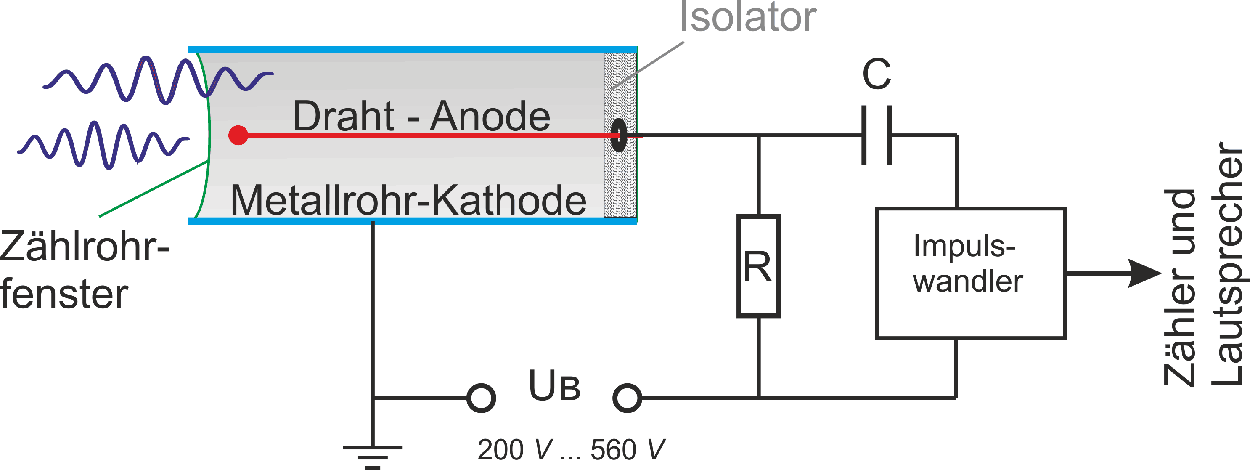
\includegraphics[height=4cm]{content/Aufbau1.png}
    \caption{Innere Perspektive des Geiger-Müller-Zählrohrs\cite{Aufbau1_GM}.}
    \label{fig:GM-Rohr}
\end{figure}

\noindent Zudem stellt die Abb. \ref{fig:GM-Rohr} dar, wie die radioaktive Strahlung duch die Folie in den Messzylinder 
eindringt. Die neutral geladenen Moleküle und Atome des Füllgases werden aufgrund der Strahlung ionisiert. Dies hat zur 
Folge, dass negativ geladenen Elektronen zum Anodendraht und positiven Ionen zum Kathodenzylinder beschleunigt werden.
Die Ionen, welche sich an der Anode bzw. Kathode sammeln, können über einen Widerstand im $\unit{\mega\ohm}$-Bereich 
abfließen, weshalb die Spannung und somit auch das elektrische Feld bei hinreichend großer Ladung stark abnimmt. 
Anschließend kann das E-Feld sukzessive wieder aufgebaut werden, sodass die nächste Strahlung detektiert werden kann.
Die nur geringfügigen Spannungsimpulse bedingen die Notwendigkeit einen Verstärker, was im Ensemble die folgende 
Versuchsapparatur ergibt:

\begin{figure}[H]
    \centering 
    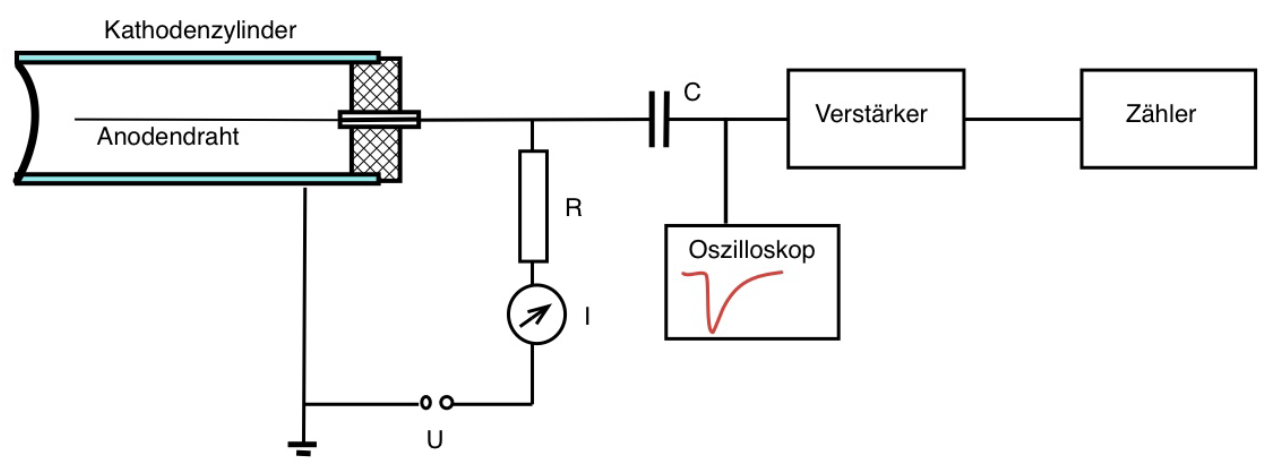
\includegraphics[height=5cm]{content/Apparatur.png}
    \caption{Versuchsapparatur des GM-Zählröhrs\cite{Versuchsanleitung_v703}}
    \label{fig:GM-Apparatur}
\end{figure}

\subsection{Geiger-Müller-Kennlinie}

\noindent Die soeben beschriebene Funktionsweise impliziert bereits eine Veränderung der \textbf{Zählrate} des Detektors bei 
einer sich veränderlichen \textbf{Betriebsspannung} zwischen Anodendraht und Messzylinder. Der Zusammenhang dieser beiden 
Größen wird als \emph{Zählrohrcharakteristik} bezeichnet. Die unten stehende Abbildung zeigt den grafischen Verlauf 
dieser sogenannten Kennlinie und ordnet die jeweiligen Intervalle definierten Bereiche zu.

\begin{figure}[H]
    \centering 
    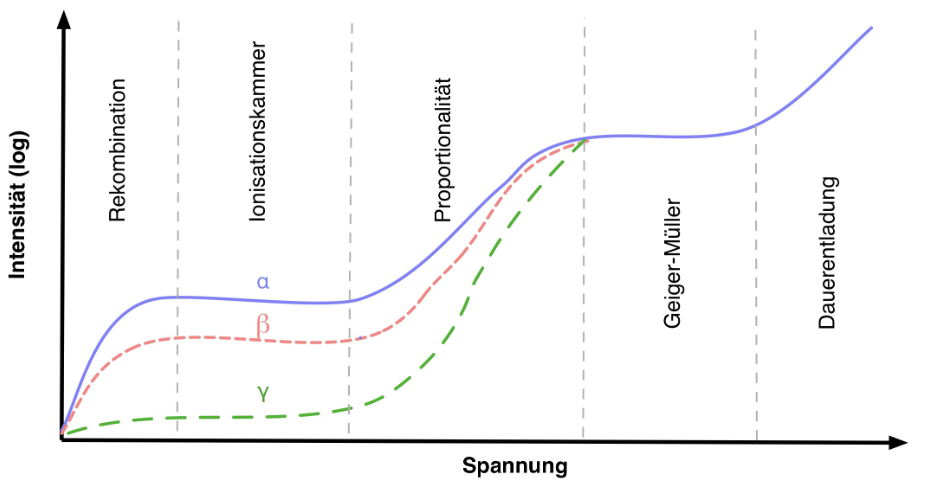
\includegraphics[height=5cm]{content/Kennlinie.png}
    \caption{Charakteristische Kennlinie eines GM-Zählrohrs\cite{KennlinieGM}}
    \label{fig:Kennlinie}
\end{figure}

\noindent Die erste Phase kleiner Betriebsspannungen wird als \textbf{Rekombination} bezeichnet. In diesem Abschnitt ist die 
Stärke des elektrischen Feldes so gering, dass sich die positiven Ionen und Elektronen während der Beschleunigungsphase verbinden
und sich somit gegenseitig neutralisieren. Bei größer werdender Spannung nimmt dieses Phänomen ab, sodass alle erzeugten 
Ionen die Elektroden erreichen können. Diese Phase wird \textbf{Ionisationskammer} genannt. Im folgenden Abschnitt des 
\textbf{Proportionalitätsbereichs} wird die Spannung weiter erhöht, sodass die Elektronen eine hinreichend große Energie 
besitzen, um durch Stoßprozesse weitere Elektronen-Ionen-Paare zu erzeugen. Diese Kettenreaktion löst ein lawinenartiges 
Verhalten um den Anodendraht aus, was teilweise zu Verstärkungsfaktoren der Zählrate im Bereich $10³$ führt. Nun folgt der 
für diesen Versuch relevante Bereich der Kennlinie. Während des sogenannten \textbf{Geiger-Müller-Bereichs} nimmt die 
Betriebsspannung so weit zu, bis Gasatome in einen angeregten Zustand versetzt werden und als Folge Photonen emittieren. 
Die Lichtquanten sind in der Lage bei direktem Zusammenstoß mit der Kathode, Photonenelektronen zu bilden, welch ebenfalls
zur Anode beschleunigt werden und die Messergebnisse verfälschen können. Während die Elektronen im Zählrohr abfließen können,
bilden die positiven Ionen eine Art \enquote{Schlauch} um den Anodendraht, welcher die Entstehung weiterer \emph{Townsend-
Lawinen} stark hemmt. Die Graphik zeigt in diesem Bereich eine nur leicht steigende Zählrate an, das sogenannte Geiger-Müller-
Plateau. Weitere Erhöhungen der Spannung führen zur \textbf{Dauerentladung} und einem drastischen Anstieg der Zählrate.

\subsection{Reale Effekte}

Neben den bereits angesprochenen Photonenelektronen treten in der Realität weitere Effekte auf, welche die Messergebnisse 
falsifizieren könnten. Beispiels entstehen beim Aufprall energiereicher Ionen mit der Kathode Sekundärelektronen, die 
zusätzliche Ausgangsimpulse hervorrufen. Zur Eindämmung dieser Effekte wird ein Löschgas eingesetzt, dessen langkettige
Moleküle die kinetische Energie der Sekundärionen aufnehmen, bevor diese zur Anode gelangen. Komplett vernachlässigt werden 
kann dieses Phänomen jedoch nicht, was im Umkehrschluss zu einer Steigung des Geiger-Müller-Plateaus führt, welche durch 
den mathematischen Ausdruck

\begin{equation}
\label{eqn:mPlateau}
    s = \frac{\increment{}N}{N}\cdot{}\qty{100}{\percent} / \qty{100}{\volt}
\end{equation}

\noindent beschrieben wird. Hierbei wird $\sfrac{\increment{}N}{N}$ als relative Zählrate pro \qty{100}{\volt} bezeichnet.\\

\noindent Sobald sich alle von der radioaktiven Strahlung freigesetzten Elektronen auf dem Anodendraht befinden senkt die 
Raumladungswolke der positiven Ionen die elektrische Feldstärke drastisch, sodass sich keine weiteren Lawinen ausbilden können.
Der GM-Zähler detektiert in diesem Zeitintervall keine Spannungsimpulse der ionisierenden Strahlung. Zunächst muss die auf dem 
Anodendraht befindliche Ladung abfließen und die Spannung erneut zunehmen, bevor eine neue Messreihe begonnen werden kann. Diese 
Zeit der Unwirksamkeit wird als \emph{Totzeit} beschrieben. Die darauf folgende \emph{Erholungszeit} beginnt mit der 
Beendigung der Totzeit und wird bei Erreichen der maximalen Zählrohrspannung terminiert. Auf dem Oszilloskop bildet sich der 
folgende ab:

\begin{figure}[H]
    \centering
    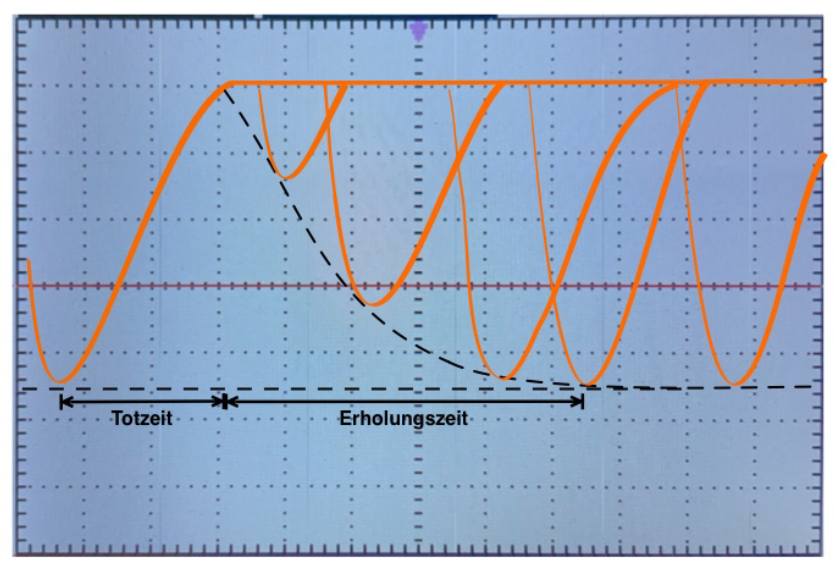
\includegraphics[height=5cm]{content/Totzeit.png}
    \caption{Tot- und Erholungszeit des GM-Zählers\cite{Versuchsanleitung_v703}.}
    \label{fig:Totzeit}
\end{figure}

\noindent Neben dem Oszilloskop kann auch die Zwei-Quellen-Methode Auskunft über die Totzeit des Detektors geben.
Die Methode beruht auf dem Zusammenhang zwischen Zählratenverlust und der Totzeit bei zunehmender Zählrate, wonach 
sich die Totzeit $\tau$ durch den Ausdruck 

\begin{equation}
\label{eqn:Totzeit}
    \tau = \frac{N_1 + N_2 - N_{12}}{2 N_1 \cdot N_2},
\end{equation}

\noindent wobei $N_1$ und $N_2$ die Zählraten der jeweiligen einzelnen Quellen und $N_{12}$ die Zählrate beider kumulierter Quellen 
beschreibt.

%\end{document}